\documentclass[1p]{elsarticle_modified}
%\bibliographystyle{elsarticle-num}

%\usepackage[colorlinks]{hyperref}
%\usepackage{abbrmath_seonhwa} %\Abb, \Ascr, \Acal ,\Abf, \Afrak
\usepackage{amsfonts}
\usepackage{amssymb}
\usepackage{amsmath}
\usepackage{amsthm}
\usepackage{scalefnt}
\usepackage{amsbsy}
\usepackage{kotex}
\usepackage{caption}
\usepackage{subfig}
\usepackage{color}
\usepackage{graphicx}
\usepackage{xcolor} %% white, black, red, green, blue, cyan, magenta, yellow
\usepackage{float}
\usepackage{setspace}
\usepackage{hyperref}

\usepackage{tikz}
\usetikzlibrary{arrows}

\usepackage{multirow}
\usepackage{array} % fixed length table
\usepackage{hhline}

%%%%%%%%%%%%%%%%%%%%%
\makeatletter
\renewcommand*\env@matrix[1][\arraystretch]{%
	\edef\arraystretch{#1}%
	\hskip -\arraycolsep
	\let\@ifnextchar\new@ifnextchar
	\array{*\c@MaxMatrixCols c}}
\makeatother %https://tex.stackexchange.com/questions/14071/how-can-i-increase-the-line-spacing-in-a-matrix
%%%%%%%%%%%%%%%

\usepackage[normalem]{ulem}

\newcommand{\msout}[1]{\ifmmode\text{\sout{\ensuremath{#1}}}\else\sout{#1}\fi}
%SOURCE: \msout is \stkout macro in https://tex.stackexchange.com/questions/20609/strikeout-in-math-mode

\newcommand{\cancel}[1]{
	\ifmmode
	{\color{red}\msout{#1}}
	\else
	{\color{red}\sout{#1}}
	\fi
}

\newcommand{\add}[1]{
	{\color{blue}\uwave{#1}}
}

\newcommand{\replace}[2]{
	\ifmmode
	{\color{red}\msout{#1}}{\color{blue}\uwave{#2}}
	\else
	{\color{red}\sout{#1}}{\color{blue}\uwave{#2}}
	\fi
}

\newcommand{\Sol}{\mathcal{S}} %segment
\newcommand{\D}{D} %diagram
\newcommand{\A}{\mathcal{A}} %arc


%%%%%%%%%%%%%%%%%%%%%%%%%%%%%5 test

\def\sl{\operatorname{\textup{SL}}(2,\Cbb)}
\def\psl{\operatorname{\textup{PSL}}(2,\Cbb)}
\def\quan{\mkern 1mu \triangleright \mkern 1mu}

\theoremstyle{definition}
\newtheorem{thm}{Theorem}[section]
\newtheorem{prop}[thm]{Proposition}
\newtheorem{lem}[thm]{Lemma}
\newtheorem{ques}[thm]{Question}
\newtheorem{cor}[thm]{Corollary}
\newtheorem{defn}[thm]{Definition}
\newtheorem{exam}[thm]{Example}
\newtheorem{rmk}[thm]{Remark}
\newtheorem{alg}[thm]{Algorithm}

\newcommand{\I}{\sqrt{-1}}
\begin{document}

%\begin{frontmatter}
%
%\title{Boundary parabolic representations of knots up to 8 crossings}
%
%%% Group authors per affiliation:
%\author{Yunhi Cho} 
%\address{Department of Mathematics, University of Seoul, Seoul, Korea}
%\ead{yhcho@uos.ac.kr}
%
%
%\author{Seonhwa Kim} %\fnref{s_kim}}
%\address{Center for Geometry and Physics, Institute for Basic Science, Pohang, 37673, Korea}
%\ead{ryeona17@ibs.re.kr}
%
%\author{Hyuk Kim}
%\address{Department of Mathematical Sciences, Seoul National University, Seoul 08826, Korea}
%\ead{hyukkim@snu.ac.kr}
%
%\author{Seokbeom Yoon}
%\address{Department of Mathematical Sciences, Seoul National University, Seoul, 08826,  Korea}
%\ead{sbyoon15@snu.ac.kr}
%
%\begin{abstract}
%We find all boundary parabolic representation of knots up to 8 crossings.
%
%\end{abstract}
%\begin{keyword}
%    \MSC[2010] 57M25 
%\end{keyword}
%
%\end{frontmatter}

%\linenumbers
%\tableofcontents
%
\newcommand\colored[1]{\textcolor{white}{\rule[-0.35ex]{0.8em}{1.4ex}}\kern-0.8em\color{red} #1}%
%\newcommand\colored[1]{\textcolor{white}{ #1}\kern-2.17ex	\textcolor{white}{ #1}\kern-1.81ex	\textcolor{white}{ #1}\kern-2.15ex\color{red}#1	}

{\Large $\underline{12n_{0080}~(K12n_{0080})}$}

\setlength{\tabcolsep}{10pt}
\renewcommand{\arraystretch}{1.6}
\vspace{1cm}\begin{tabular}{m{100pt}>{\centering\arraybackslash}m{274pt}}
\multirow{5}{120pt}{
	\centering
	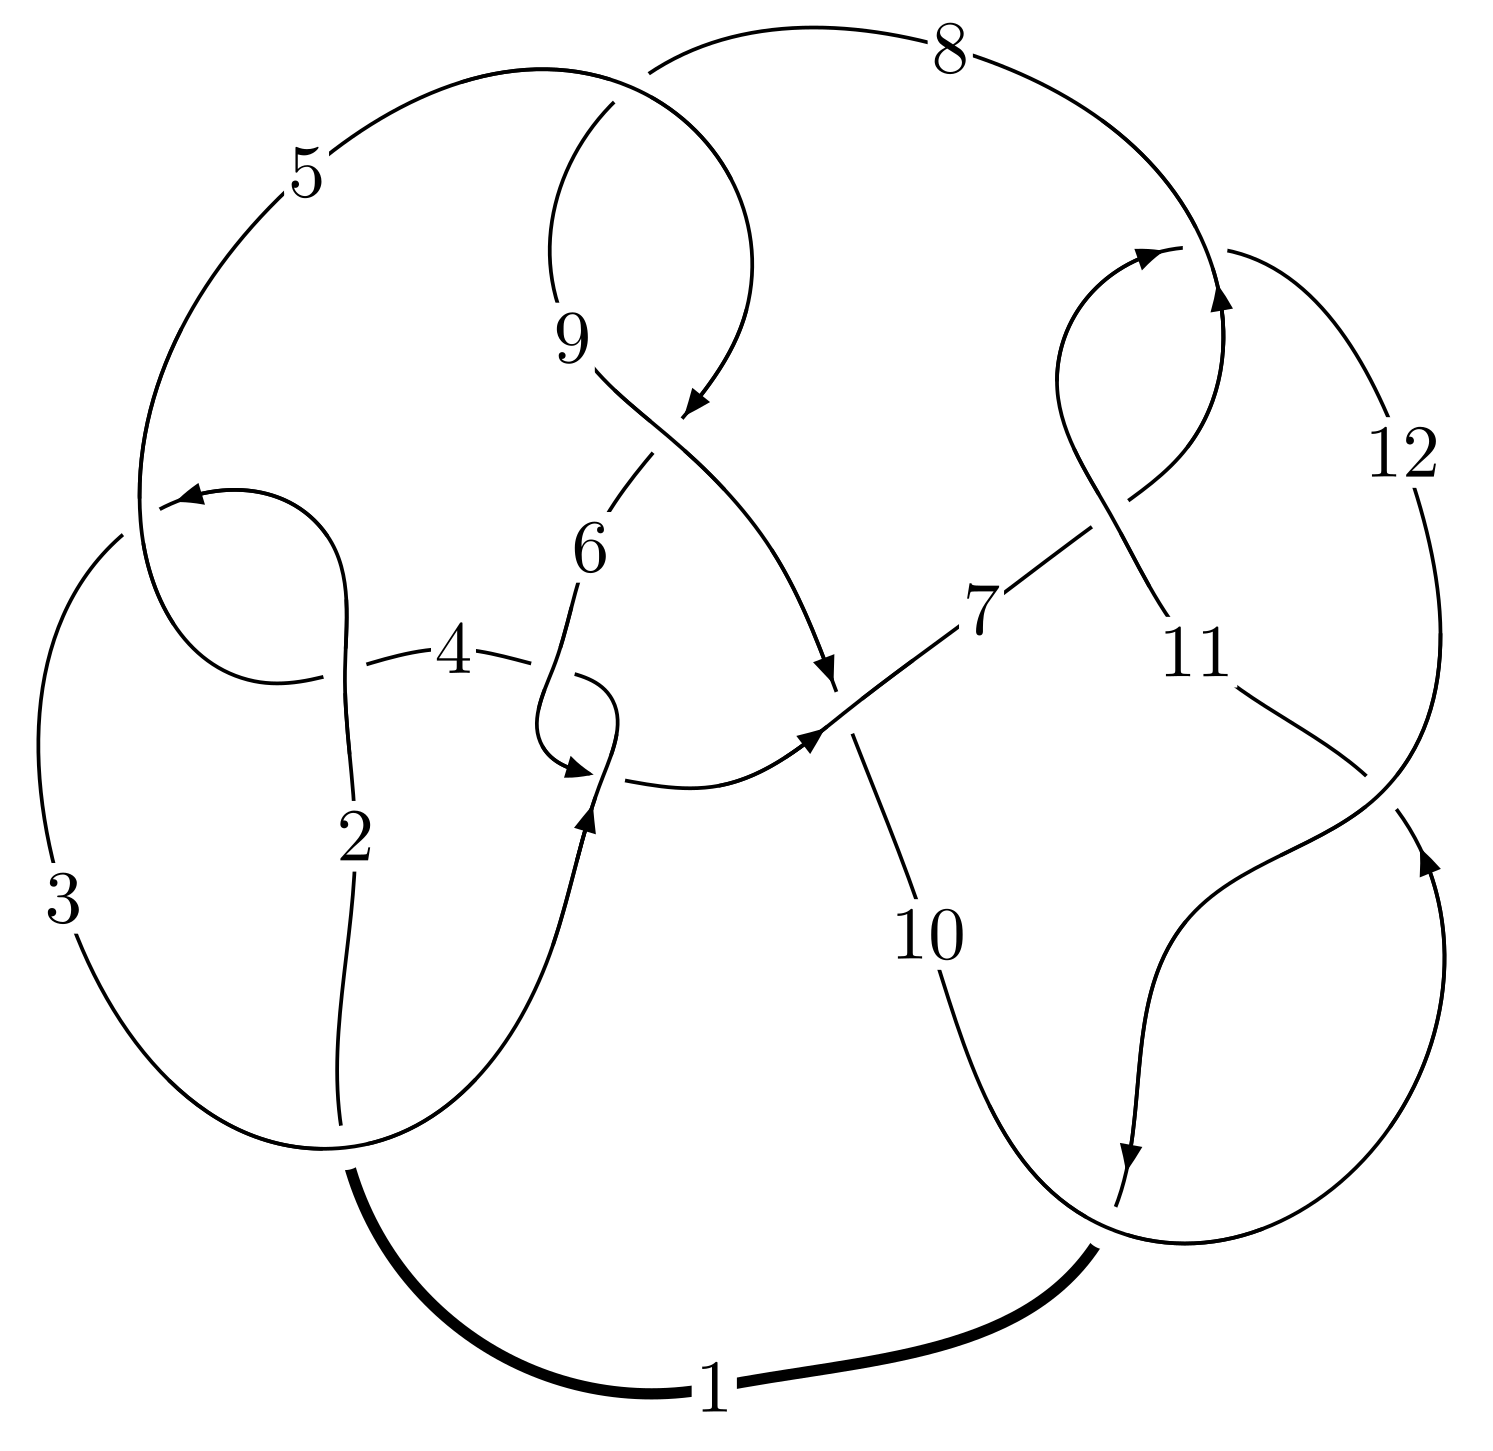
\includegraphics[width=112pt]{../../../GIT/diagram.site/Diagrams/png/2169_12n_0080.png}\\
\ \ \ A knot diagram\footnotemark}&
\allowdisplaybreaks
\textbf{Linearized knot diagam} \\
\cline{2-2}
 &
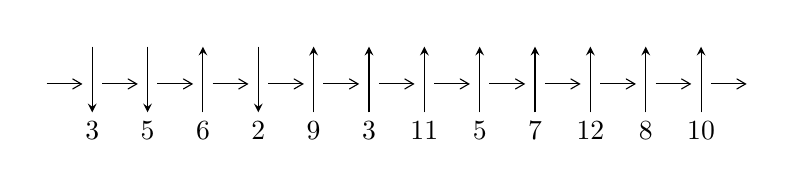
\begin{tikzpicture}[x=20pt, y=17pt]
	% nodes
	\node (C0) at (0, 0) {};
	\node (C1) at (1, 0) {};
	\node (C1U) at (1, +1) {};
	\node (C1D) at (1, -1) {3};

	\node (C2) at (2, 0) {};
	\node (C2U) at (2, +1) {};
	\node (C2D) at (2, -1) {5};

	\node (C3) at (3, 0) {};
	\node (C3U) at (3, +1) {};
	\node (C3D) at (3, -1) {6};

	\node (C4) at (4, 0) {};
	\node (C4U) at (4, +1) {};
	\node (C4D) at (4, -1) {2};

	\node (C5) at (5, 0) {};
	\node (C5U) at (5, +1) {};
	\node (C5D) at (5, -1) {9};

	\node (C6) at (6, 0) {};
	\node (C6U) at (6, +1) {};
	\node (C6D) at (6, -1) {3};

	\node (C7) at (7, 0) {};
	\node (C7U) at (7, +1) {};
	\node (C7D) at (7, -1) {11};

	\node (C8) at (8, 0) {};
	\node (C8U) at (8, +1) {};
	\node (C8D) at (8, -1) {5};

	\node (C9) at (9, 0) {};
	\node (C9U) at (9, +1) {};
	\node (C9D) at (9, -1) {7};

	\node (C10) at (10, 0) {};
	\node (C10U) at (10, +1) {};
	\node (C10D) at (10, -1) {12};

	\node (C11) at (11, 0) {};
	\node (C11U) at (11, +1) {};
	\node (C11D) at (11, -1) {8};

	\node (C12) at (12, 0) {};
	\node (C12U) at (12, +1) {};
	\node (C12D) at (12, -1) {10};
	\node (C13) at (13, 0) {};

	% arrows
	\draw[->,>={angle 60}]
	(C0) edge (C1) (C1) edge (C2) (C2) edge (C3) (C3) edge (C4) (C4) edge (C5) (C5) edge (C6) (C6) edge (C7) (C7) edge (C8) (C8) edge (C9) (C9) edge (C10) (C10) edge (C11) (C11) edge (C12) (C12) edge (C13) ;	\draw[->,>=stealth]
	(C1U) edge (C1D) (C2U) edge (C2D) (C3D) edge (C3U) (C4U) edge (C4D) (C5D) edge (C5U) (C6D) edge (C6U) (C7D) edge (C7U) (C8D) edge (C8U) (C9D) edge (C9U) (C10D) edge (C10U) (C11D) edge (C11U) (C12D) edge (C12U) ;
	\end{tikzpicture} \\
\hhline{~~} \\& 
\textbf{Solving Sequence} \\ \cline{2-2} 
 &
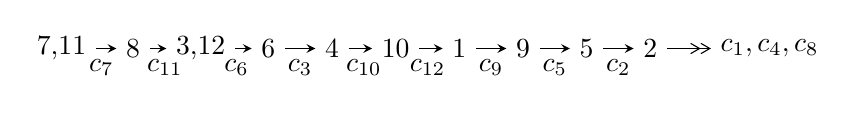
\begin{tikzpicture}[x=23pt, y=7pt]
	% node
	\node (A0) at (-1/8, 0) {7,11};
	\node (A1) at (1, 0) {8};
	\node (A2) at (33/16, 0) {3,12};
	\node (A3) at (25/8, 0) {6};
	\node (A4) at (33/8, 0) {4};
	\node (A5) at (41/8, 0) {10};
	\node (A6) at (49/8, 0) {1};
	\node (A7) at (57/8, 0) {9};
	\node (A8) at (65/8, 0) {5};
	\node (A9) at (73/8, 0) {2};
	\node (C1) at (1/2, -1) {$c_{7}$};
	\node (C2) at (3/2, -1) {$c_{11}$};
	\node (C3) at (21/8, -1) {$c_{6}$};
	\node (C4) at (29/8, -1) {$c_{3}$};
	\node (C5) at (37/8, -1) {$c_{10}$};
	\node (C6) at (45/8, -1) {$c_{12}$};
	\node (C7) at (53/8, -1) {$c_{9}$};
	\node (C8) at (61/8, -1) {$c_{5}$};
	\node (C9) at (69/8, -1) {$c_{2}$};
	\node (A10) at (11, 0) {$c_{1},c_{4},c_{8}$};

	% edge
	\draw[->,>=stealth]	
	(A0) edge (A1) (A1) edge (A2) (A2) edge (A3) (A3) edge (A4) (A4) edge (A5) (A5) edge (A6) (A6) edge (A7) (A7) edge (A8) (A8) edge (A9) ;
	\draw[->>,>={angle 60}]	
	(A9) edge (A10);
\end{tikzpicture} \\ 

\end{tabular} \\

\footnotetext{
The image of knot diagram is generated by the software ``\textbf{Draw programme}" developed by Andrew Bartholomew(\url{http://www.layer8.co.uk/maths/draw/index.htm\#Running-draw}), where we modified some parts for our purpose(\url{https://github.com/CATsTAILs/LinksPainter}).
}\phantom \\ \newline 
\centering \textbf{Ideals for irreducible components\footnotemark of $X_{\text{par}}$} 
 
\begin{align*}
I^u_{1}&=\langle 
11188446734 u^{40}+14624888210 u^{39}+\cdots+38482965369 b-18882609362,\\
\phantom{I^u_{1}}&\phantom{= \langle  }-471858393299 u^{40}-603105686012 u^{39}+\cdots+38482965369 a+737953573358,\\
\phantom{I^u_{1}}&\phantom{= \langle  }u^{41}+2 u^{40}+\cdots- u-1\rangle \\
I^u_{2}&=\langle 
b,\;3 u^7+u^6-4 u^5-4 u^4+5 u^3+3 u^2+a- u-5,\;u^8+u^7- u^6-2 u^5+u^4+2 u^3-2 u-1\rangle \\
\\
\end{align*}
\raggedright * 2 irreducible components of $\dim_{\mathbb{C}}=0$, with total 49 representations.\\
\footnotetext{All coefficients of polynomials are rational numbers. But the coefficients are sometimes approximated in decimal forms when there is not enough margin.}
\newpage
\renewcommand{\arraystretch}{1}
\centering \section*{I. $I^u_{1}= \langle 1.12\times10^{10} u^{40}+1.46\times10^{10} u^{39}+\cdots+3.85\times10^{10} b-1.89\times10^{10},\;-4.72\times10^{11} u^{40}-6.03\times10^{11} u^{39}+\cdots+3.85\times10^{10} a+7.38\times10^{11},\;u^{41}+2 u^{40}+\cdots- u-1 \rangle$}
\flushleft \textbf{(i) Arc colorings}\\
\begin{tabular}{m{7pt} m{180pt} m{7pt} m{180pt} }
\flushright $a_{7}=$&$\begin{pmatrix}1\\0\end{pmatrix}$ \\
\flushright $a_{11}=$&$\begin{pmatrix}0\\u\end{pmatrix}$ \\
\flushright $a_{8}=$&$\begin{pmatrix}1\\- u^2\end{pmatrix}$ \\
\flushright $a_{3}=$&$\begin{pmatrix}12.2615 u^{40}+15.6720 u^{39}+\cdots+6.84293 u-19.1761\\-0.290738 u^{40}-0.380035 u^{39}+\cdots+1.44537 u+0.490674\end{pmatrix}$ \\
\flushright $a_{12}=$&$\begin{pmatrix}u\\- u^3+u\end{pmatrix}$ \\
\flushright $a_{6}=$&$\begin{pmatrix}-3.45682 u^{40}-4.64440 u^{39}+\cdots-4.50872 u+4.12223\\0.869179 u^{40}+1.73038 u^{39}+\cdots-0.134593 u-0.868998\end{pmatrix}$ \\
\flushright $a_{4}=$&$\begin{pmatrix}9.93735 u^{40}+13.3319 u^{39}+\cdots+8.96828 u-18.9057\\2.61664 u^{40}+5.42032 u^{39}+\cdots-0.00831753 u-2.41607\end{pmatrix}$ \\
\flushright $a_{10}=$&$\begin{pmatrix}- u^3\\u^5- u^3+u\end{pmatrix}$ \\
\flushright $a_{1}=$&$\begin{pmatrix}u^5+u\\- u^7+u^5-2 u^3+u\end{pmatrix}$ \\
\flushright $a_{9}=$&$\begin{pmatrix}- u^5- u\\u^5- u^3+u\end{pmatrix}$ \\
\flushright $a_{5}=$&$\begin{pmatrix}-2.06817 u^{40}-2.86404 u^{39}+\cdots-3.90693 u+2.53206\\-0.127787 u^{40}+0.140106 u^{39}+\cdots-0.336106 u+0.527977\end{pmatrix}$ \\
\flushright $a_{2}=$&$\begin{pmatrix}10.3978 u^{40}+13.4001 u^{39}+\cdots+5.65679 u-18.2402\\0.964836 u^{40}+2.33975 u^{39}+\cdots+1.11758 u-0.565279\end{pmatrix}$\\&\end{tabular}
\flushleft \textbf{(ii) Obstruction class $= -1$}\\~\\
\flushleft \textbf{(iii) Cusp Shapes $= \frac{1507194298715}{12827655123} u^{40}+\frac{1944574441589}{12827655123} u^{39}+\cdots+\frac{274922951097}{4275885041} u-\frac{2104450199471}{12827655123}$}\\~\\
\newpage\renewcommand{\arraystretch}{1}
\flushleft \textbf{(iv) u-Polynomials at the component}\newline \\
\begin{tabular}{m{50pt}|m{274pt}}
Crossings & \hspace{64pt}u-Polynomials at each crossing \\
\hline $$\begin{aligned}c_{1}\end{aligned}$$&$\begin{aligned}
&u^{41}+53 u^{40}+\cdots+381 u+1
\end{aligned}$\\
\hline $$\begin{aligned}c_{2},c_{4}\end{aligned}$$&$\begin{aligned}
&u^{41}-9 u^{40}+\cdots-29 u+1
\end{aligned}$\\
\hline $$\begin{aligned}c_{3},c_{6}\end{aligned}$$&$\begin{aligned}
&u^{41}+7 u^{40}+\cdots+2176 u-256
\end{aligned}$\\
\hline $$\begin{aligned}c_{5},c_{8}\end{aligned}$$&$\begin{aligned}
&u^{41}-2 u^{40}+\cdots+u-1
\end{aligned}$\\
\hline $$\begin{aligned}c_{7},c_{11}\end{aligned}$$&$\begin{aligned}
&u^{41}-2 u^{40}+\cdots- u+1
\end{aligned}$\\
\hline $$\begin{aligned}c_{9}\end{aligned}$$&$\begin{aligned}
&u^{41}+2 u^{40}+\cdots+12241 u+8353
\end{aligned}$\\
\hline $$\begin{aligned}c_{10},c_{12}\end{aligned}$$&$\begin{aligned}
&u^{41}-12 u^{40}+\cdots+5 u-1
\end{aligned}$\\
\hline
\end{tabular}\\~\\
\newpage\renewcommand{\arraystretch}{1}
\flushleft \textbf{(v) Riley Polynomials at the component}\newline \\
\begin{tabular}{m{50pt}|m{274pt}}
Crossings & \hspace{64pt}Riley Polynomials at each crossing \\
\hline $$\begin{aligned}c_{1}\end{aligned}$$&$\begin{aligned}
&y^{41}-121 y^{40}+\cdots+73433 y-1
\end{aligned}$\\
\hline $$\begin{aligned}c_{2},c_{4}\end{aligned}$$&$\begin{aligned}
&y^{41}-53 y^{40}+\cdots+381 y-1
\end{aligned}$\\
\hline $$\begin{aligned}c_{3},c_{6}\end{aligned}$$&$\begin{aligned}
&y^{41}+51 y^{40}+\cdots+2801664 y-65536
\end{aligned}$\\
\hline $$\begin{aligned}c_{5},c_{8}\end{aligned}$$&$\begin{aligned}
&y^{41}+42 y^{39}+\cdots+5 y-1
\end{aligned}$\\
\hline $$\begin{aligned}c_{7},c_{11}\end{aligned}$$&$\begin{aligned}
&y^{41}-12 y^{40}+\cdots+5 y-1
\end{aligned}$\\
\hline $$\begin{aligned}c_{9}\end{aligned}$$&$\begin{aligned}
&y^{41}+36 y^{40}+\cdots+949291005 y-69772609
\end{aligned}$\\
\hline $$\begin{aligned}c_{10},c_{12}\end{aligned}$$&$\begin{aligned}
&y^{41}+36 y^{40}+\cdots+37 y-1
\end{aligned}$\\
\hline
\end{tabular}\\~\\
\newpage\flushleft \textbf{(vi) Complex Volumes and Cusp Shapes}
$$\begin{array}{c|c|c}  
\text{Solutions to }I^u_{1}& \I (\text{vol} + \sqrt{-1}CS) & \text{Cusp shape}\\
 \hline 
\begin{aligned}
u &= -0.645157 + 0.706341 I \\
a &= \phantom{-}0.129346 + 0.199509 I \\
b &= -0.707026 - 0.083217 I\end{aligned}
 & \phantom{-}0.314025 + 0.700329 I & \phantom{-}9.78155 + 0.42575 I \\ \hline\begin{aligned}
u &= -0.645157 - 0.706341 I \\
a &= \phantom{-}0.129346 - 0.199509 I \\
b &= -0.707026 + 0.083217 I\end{aligned}
 & \phantom{-}0.314025 - 0.700329 I & \phantom{-}9.78155 - 0.42575 I \\ \hline\begin{aligned}
u &= \phantom{-}1.06514\phantom{ +0.000000I} \\
a &= \phantom{-}1.21465\phantom{ +0.000000I} \\
b &= -0.619887\phantom{ +0.000000I}\end{aligned}
 & \phantom{-}5.55858\phantom{ +0.000000I} & \phantom{-}18.6510\phantom{ +0.000000I} \\ \hline\begin{aligned}
u &= \phantom{-}0.878483 + 0.257640 I \\
a &= \phantom{-}1.36190 + 1.41715 I \\
b &= -0.395484 - 1.274730 I\end{aligned}
 & \phantom{-}0.35281 + 3.72015 I & \phantom{-}8.01877 - 8.67695 I \\ \hline\begin{aligned}
u &= \phantom{-}0.878483 - 0.257640 I \\
a &= \phantom{-}1.36190 - 1.41715 I \\
b &= -0.395484 + 1.274730 I\end{aligned}
 & \phantom{-}0.35281 - 3.72015 I & \phantom{-}8.01877 + 8.67695 I \\ \hline\begin{aligned}
u &= \phantom{-}0.863822 + 0.692291 I \\
a &= -0.710177 + 0.248903 I \\
b &= \phantom{-}0.360833 - 0.064088 I\end{aligned}
 & -2.33978 + 2.66185 I & \phantom{-}4.87613 - 3.55699 I \\ \hline\begin{aligned}
u &= \phantom{-}0.863822 - 0.692291 I \\
a &= -0.710177 - 0.248903 I \\
b &= \phantom{-}0.360833 + 0.064088 I\end{aligned}
 & -2.33978 - 2.66185 I & \phantom{-}4.87613 + 3.55699 I \\ \hline\begin{aligned}
u &= \phantom{-}0.850650 + 0.773602 I \\
a &= \phantom{-}0.65587 - 1.74300 I \\
b &= -0.305447 - 0.669138 I\end{aligned}
 & -4.76432 + 2.07222 I & \phantom{-}3.47881 - 9.56031 I \\ \hline\begin{aligned}
u &= \phantom{-}0.850650 - 0.773602 I \\
a &= \phantom{-}0.65587 + 1.74300 I \\
b &= -0.305447 + 0.669138 I\end{aligned}
 & -4.76432 - 2.07222 I & \phantom{-}3.47881 + 9.56031 I \\ \hline\begin{aligned}
u &= \phantom{-}1.113340 + 0.298427 I \\
a &= -2.09473 - 1.98305 I \\
b &= \phantom{-}0.58426 + 1.64109 I\end{aligned}
 & -6.81237 + 7.94638 I & \phantom{-}6.00000 - 5.66643 I\\
 \hline 
 \end{array}$$\newpage$$\begin{array}{c|c|c}  
\text{Solutions to }I^u_{1}& \I (\text{vol} + \sqrt{-1}CS) & \text{Cusp shape}\\
 \hline 
\begin{aligned}
u &= \phantom{-}1.113340 - 0.298427 I \\
a &= -2.09473 + 1.98305 I \\
b &= \phantom{-}0.58426 - 1.64109 I\end{aligned}
 & -6.81237 - 7.94638 I & \phantom{-}6.00000 + 5.66643 I \\ \hline\begin{aligned}
u &= -1.123200 + 0.281615 I \\
a &= \phantom{-}0.82820 - 2.54731 I \\
b &= \phantom{-}0.17091 + 1.62625 I\end{aligned}
 & -6.69343 + 0.45475 I & \phantom{-}6.00000 + 0.74518 I \\ \hline\begin{aligned}
u &= -1.123200 - 0.281615 I \\
a &= \phantom{-}0.82820 + 2.54731 I \\
b &= \phantom{-}0.17091 - 1.62625 I\end{aligned}
 & -6.69343 - 0.45475 I & \phantom{-}6.00000 - 0.74518 I \\ \hline\begin{aligned}
u &= -0.821741 + 0.155454 I \\
a &= -1.49310 + 0.28695 I \\
b &= \phantom{-}0.000254 - 0.581031 I\end{aligned}
 & \phantom{-}0.614586 - 0.353193 I & \phantom{-}8.75569 + 0.62140 I \\ \hline\begin{aligned}
u &= -0.821741 - 0.155454 I \\
a &= -1.49310 - 0.28695 I \\
b &= \phantom{-}0.000254 + 0.581031 I\end{aligned}
 & \phantom{-}0.614586 + 0.353193 I & \phantom{-}8.75569 - 0.62140 I \\ \hline\begin{aligned}
u &= -0.829859 + 0.817277 I \\
a &= -1.080080 - 0.171992 I \\
b &= \phantom{-}0.03664 - 2.09736 I\end{aligned}
 & -6.22251 + 1.37166 I & \phantom{-0.000000 } 0. - 2.74151 I \\ \hline\begin{aligned}
u &= -0.829859 - 0.817277 I \\
a &= -1.080080 + 0.171992 I \\
b &= \phantom{-}0.03664 + 2.09736 I\end{aligned}
 & -6.22251 - 1.37166 I & \phantom{-0.000000 -}0. + 2.74151 I \\ \hline\begin{aligned}
u &= \phantom{-}0.739042 + 0.910928 I \\
a &= -0.097736 - 0.296625 I \\
b &= -0.10739 + 1.92349 I\end{aligned}
 & -14.7874 + 0.6933 I & \phantom{-0.000000 } 0. - 1.66266 I \\ \hline\begin{aligned}
u &= \phantom{-}0.739042 - 0.910928 I \\
a &= -0.097736 + 0.296625 I \\
b &= -0.10739 - 1.92349 I\end{aligned}
 & -14.7874 - 0.6933 I & \phantom{-0.000000 -}0. + 1.66266 I \\ \hline\begin{aligned}
u &= -0.746747 + 0.906172 I \\
a &= -0.099105 - 0.285226 I \\
b &= \phantom{-}0.82858 + 1.91790 I\end{aligned}
 & -14.9445 + 7.5314 I & \phantom{-0.000000 } 0. - 2.54363 I\\
 \hline 
 \end{array}$$\newpage$$\begin{array}{c|c|c}  
\text{Solutions to }I^u_{1}& \I (\text{vol} + \sqrt{-1}CS) & \text{Cusp shape}\\
 \hline 
\begin{aligned}
u &= -0.746747 - 0.906172 I \\
a &= -0.099105 + 0.285226 I \\
b &= \phantom{-}0.82858 - 1.91790 I\end{aligned}
 & -14.9445 - 7.5314 I & \phantom{-0.000000 -}0. + 2.54363 I \\ \hline\begin{aligned}
u &= \phantom{-}0.010347 + 0.818382 I \\
a &= -0.096572 + 0.286828 I \\
b &= \phantom{-}0.37826 - 1.80255 I\end{aligned}
 & -10.51980 - 4.16733 I & \phantom{-}0.66529 + 2.27689 I \\ \hline\begin{aligned}
u &= \phantom{-}0.010347 - 0.818382 I \\
a &= -0.096572 - 0.286828 I \\
b &= \phantom{-}0.37826 + 1.80255 I\end{aligned}
 & -10.51980 + 4.16733 I & \phantom{-}0.66529 - 2.27689 I \\ \hline\begin{aligned}
u &= \phantom{-}0.913540 + 0.760932 I \\
a &= -0.676289 + 1.093800 I \\
b &= -0.209840 + 0.757944 I\end{aligned}
 & -4.56999 + 3.72466 I & \phantom{-}3.33454 + 2.09517 I \\ \hline\begin{aligned}
u &= \phantom{-}0.913540 - 0.760932 I \\
a &= -0.676289 - 1.093800 I \\
b &= -0.209840 - 0.757944 I\end{aligned}
 & -4.56999 - 3.72466 I & \phantom{-}3.33454 - 2.09517 I \\ \hline\begin{aligned}
u &= -0.893232 + 0.810220 I \\
a &= -0.95737 - 1.53330 I \\
b &= \phantom{-}2.34407 + 0.13131 I\end{aligned}
 & -8.47280 - 3.03045 I & \phantom{-0.000000 -}0. + 2.81396 I \\ \hline\begin{aligned}
u &= -0.893232 - 0.810220 I \\
a &= -0.95737 + 1.53330 I \\
b &= \phantom{-}2.34407 - 0.13131 I\end{aligned}
 & -8.47280 + 3.03045 I & \phantom{-0.000000 } 0. - 2.81396 I \\ \hline\begin{aligned}
u &= -1.010010 + 0.669120 I \\
a &= \phantom{-}0.541263 + 0.790129 I \\
b &= -0.710082 - 0.023150 I\end{aligned}
 & \phantom{-}1.39688 - 6.02924 I & \phantom{-}12.17156 + 3.37002 I \\ \hline\begin{aligned}
u &= -1.010010 - 0.669120 I \\
a &= \phantom{-}0.541263 - 0.790129 I \\
b &= -0.710082 + 0.023150 I\end{aligned}
 & \phantom{-}1.39688 + 6.02924 I & \phantom{-}12.17156 - 3.37002 I \\ \hline\begin{aligned}
u &= -0.944017 + 0.784096 I \\
a &= \phantom{-}1.80124 - 0.03860 I \\
b &= -0.19373 + 2.11976 I\end{aligned}
 & -5.86990 - 7.37157 I & \phantom{-}6.00000 + 8.00321 I\\
 \hline 
 \end{array}$$\newpage$$\begin{array}{c|c|c}  
\text{Solutions to }I^u_{1}& \I (\text{vol} + \sqrt{-1}CS) & \text{Cusp shape}\\
 \hline 
\begin{aligned}
u &= -0.944017 - 0.784096 I \\
a &= \phantom{-}1.80124 + 0.03860 I \\
b &= -0.19373 - 2.11976 I\end{aligned}
 & -5.86990 + 7.37157 I & \phantom{-}6.00000 - 8.00321 I \\ \hline\begin{aligned}
u &= -1.028850 + 0.790391 I \\
a &= -2.50865 - 0.19833 I \\
b &= \phantom{-}0.91594 - 1.85439 I\end{aligned}
 & -14.0605 - 13.8029 I & \phantom{-0.000000 } 0 \\ \hline\begin{aligned}
u &= -1.028850 - 0.790391 I \\
a &= -2.50865 + 0.19833 I \\
b &= \phantom{-}0.91594 + 1.85439 I\end{aligned}
 & -14.0605 + 13.8029 I & \phantom{-0.000000 } 0 \\ \hline\begin{aligned}
u &= \phantom{-}1.035690 + 0.788962 I \\
a &= \phantom{-}2.07595 + 0.63512 I \\
b &= -0.21521 - 1.85036 I\end{aligned}
 & -13.8581 + 5.5876 I & \phantom{-0.000000 } 0 \\ \hline\begin{aligned}
u &= \phantom{-}1.035690 - 0.788962 I \\
a &= \phantom{-}2.07595 - 0.63512 I \\
b &= -0.21521 + 1.85036 I\end{aligned}
 & -13.8581 - 5.5876 I & \phantom{-0.000000 } 0 \\ \hline\begin{aligned}
u &= -0.691121\phantom{ +0.000000I} \\
a &= \phantom{-}7.56339\phantom{ +0.000000I} \\
b &= -0.229386\phantom{ +0.000000I}\end{aligned}
 & -0.704951\phantom{ +0.000000I} & \phantom{-}91.2610\phantom{ +0.000000I} \\ \hline\begin{aligned}
u &= \phantom{-}0.593654 + 0.309854 I \\
a &= -2.47422 + 0.91083 I \\
b &= \phantom{-}1.073020 - 0.556578 I\end{aligned}
 & -2.54134 + 1.31981 I & \phantom{-}0.58683 - 4.31452 I \\ \hline\begin{aligned}
u &= \phantom{-}0.593654 - 0.309854 I \\
a &= -2.47422 - 0.91083 I \\
b &= \phantom{-}1.073020 + 0.556578 I\end{aligned}
 & -2.54134 - 1.31981 I & \phantom{-}0.58683 + 4.31452 I \\ \hline\begin{aligned}
u &= -0.530048\phantom{ +0.000000I} \\
a &= -0.522918\phantom{ +0.000000I} \\
b &= -0.246323\phantom{ +0.000000I}\end{aligned}
 & \phantom{-}0.790977\phantom{ +0.000000I} & \phantom{-}12.7730\phantom{ +0.000000I} \\ \hline\begin{aligned}
u &= \phantom{-}0.122257 + 0.387519 I \\
a &= -1.73330 + 0.73700 I \\
b &= \phantom{-}0.199239 + 0.977182 I\end{aligned}
 & -1.72184 - 1.26203 I & -0.75083 + 2.53377 I\\
 \hline 
 \end{array}$$\newpage$$\begin{array}{c|c|c}  
\text{Solutions to }I^u_{1}& \I (\text{vol} + \sqrt{-1}CS) & \text{Cusp shape}\\
 \hline 
\begin{aligned}
u &= \phantom{-}0.122257 - 0.387519 I \\
a &= -1.73330 - 0.73700 I \\
b &= \phantom{-}0.199239 - 0.977182 I\end{aligned}
 & -1.72184 + 1.26203 I & -0.75083 - 2.53377 I\\
 \hline 
 \end{array}$$\newpage\newpage\renewcommand{\arraystretch}{1}
\centering \section*{II. $I^u_{2}= \langle b,\;3 u^7+u^6-4 u^5-4 u^4+5 u^3+3 u^2+a- u-5,\;u^8+u^7- u^6-2 u^5+u^4+2 u^3-2 u-1 \rangle$}
\flushleft \textbf{(i) Arc colorings}\\
\begin{tabular}{m{7pt} m{180pt} m{7pt} m{180pt} }
\flushright $a_{7}=$&$\begin{pmatrix}1\\0\end{pmatrix}$ \\
\flushright $a_{11}=$&$\begin{pmatrix}0\\u\end{pmatrix}$ \\
\flushright $a_{8}=$&$\begin{pmatrix}1\\- u^2\end{pmatrix}$ \\
\flushright $a_{3}=$&$\begin{pmatrix}-3 u^7- u^6+4 u^5+4 u^4-5 u^3-3 u^2+u+5\\0\end{pmatrix}$ \\
\flushright $a_{12}=$&$\begin{pmatrix}u\\- u^3+u\end{pmatrix}$ \\
\flushright $a_{6}=$&$\begin{pmatrix}1\\0\end{pmatrix}$ \\
\flushright $a_{4}=$&$\begin{pmatrix}-3 u^7- u^6+4 u^5+4 u^4-5 u^3-3 u^2+u+5\\0\end{pmatrix}$ \\
\flushright $a_{10}=$&$\begin{pmatrix}- u^3\\u^5- u^3+u\end{pmatrix}$ \\
\flushright $a_{1}=$&$\begin{pmatrix}u^5+u\\- u^7+u^5-2 u^3+u\end{pmatrix}$ \\
\flushright $a_{9}=$&$\begin{pmatrix}- u^5- u\\u^5- u^3+u\end{pmatrix}$ \\
\flushright $a_{5}=$&$\begin{pmatrix}- u^5- u\\u^7- u^5+2 u^3- u\end{pmatrix}$ \\
\flushright $a_{2}=$&$\begin{pmatrix}-3 u^7- u^6+5 u^5+4 u^4-5 u^3-3 u^2+2 u+5\\- u^7+u^5-2 u^3+u\end{pmatrix}$\\&\end{tabular}
\flushleft \textbf{(ii) Obstruction class $= 1$}\\~\\
\flushleft \textbf{(iii) Cusp Shapes $= 9 u^7+6 u^6-8 u^5-14 u^4+15 u^3+9 u^2-4 u-15$}\\~\\
\newpage\renewcommand{\arraystretch}{1}
\flushleft \textbf{(iv) u-Polynomials at the component}\newline \\
\begin{tabular}{m{50pt}|m{274pt}}
Crossings & \hspace{64pt}u-Polynomials at each crossing \\
\hline $$\begin{aligned}c_{1},c_{2}\end{aligned}$$&$\begin{aligned}
&(u-1)^8
\end{aligned}$\\
\hline $$\begin{aligned}c_{3},c_{6}\end{aligned}$$&$\begin{aligned}
&u^8
\end{aligned}$\\
\hline $$\begin{aligned}c_{4}\end{aligned}$$&$\begin{aligned}
&(u+1)^8
\end{aligned}$\\
\hline $$\begin{aligned}c_{5}\end{aligned}$$&$\begin{aligned}
&u^8- u^7-3 u^6+2 u^5+3 u^4-2 u-1
\end{aligned}$\\
\hline $$\begin{aligned}c_{7}\end{aligned}$$&$\begin{aligned}
&u^8+u^7- u^6-2 u^5+u^4+2 u^3-2 u-1
\end{aligned}$\\
\hline $$\begin{aligned}c_{8},c_{9}\end{aligned}$$&$\begin{aligned}
&u^8+u^7-3 u^6-2 u^5+3 u^4+2 u-1
\end{aligned}$\\
\hline $$\begin{aligned}c_{10}\end{aligned}$$&$\begin{aligned}
&u^8+3 u^7+7 u^6+10 u^5+11 u^4+10 u^3+6 u^2+4 u+1
\end{aligned}$\\
\hline $$\begin{aligned}c_{11}\end{aligned}$$&$\begin{aligned}
&u^8- u^7- u^6+2 u^5+u^4-2 u^3+2 u-1
\end{aligned}$\\
\hline $$\begin{aligned}c_{12}\end{aligned}$$&$\begin{aligned}
&u^8-3 u^7+7 u^6-10 u^5+11 u^4-10 u^3+6 u^2-4 u+1
\end{aligned}$\\
\hline
\end{tabular}\\~\\
\newpage\renewcommand{\arraystretch}{1}
\flushleft \textbf{(v) Riley Polynomials at the component}\newline \\
\begin{tabular}{m{50pt}|m{274pt}}
Crossings & \hspace{64pt}Riley Polynomials at each crossing \\
\hline $$\begin{aligned}c_{1},c_{2},c_{4}\end{aligned}$$&$\begin{aligned}
&(y-1)^8
\end{aligned}$\\
\hline $$\begin{aligned}c_{3},c_{6}\end{aligned}$$&$\begin{aligned}
&y^8
\end{aligned}$\\
\hline $$\begin{aligned}c_{5},c_{8},c_{9}\end{aligned}$$&$\begin{aligned}
&y^8-7 y^7+19 y^6-22 y^5+3 y^4+14 y^3-6 y^2-4 y+1
\end{aligned}$\\
\hline $$\begin{aligned}c_{7},c_{11}\end{aligned}$$&$\begin{aligned}
&y^8-3 y^7+7 y^6-10 y^5+11 y^4-10 y^3+6 y^2-4 y+1
\end{aligned}$\\
\hline $$\begin{aligned}c_{10},c_{12}\end{aligned}$$&$\begin{aligned}
&y^8+5 y^7+11 y^6+6 y^5-17 y^4-34 y^3-22 y^2-4 y+1
\end{aligned}$\\
\hline
\end{tabular}\\~\\
\newpage\flushleft \textbf{(vi) Complex Volumes and Cusp Shapes}
$$\begin{array}{c|c|c}  
\text{Solutions to }I^u_{2}& \I (\text{vol} + \sqrt{-1}CS) & \text{Cusp shape}\\
 \hline 
\begin{aligned}
u &= -0.570868 + 0.730671 I \\
a &= \phantom{-}0.615431 - 0.295452 I \\
b &= \phantom{-0.000000 } 0\end{aligned}
 & -0.604279 + 1.131230 I & \phantom{-}1.78185 - 1.82144 I \\ \hline\begin{aligned}
u &= -0.570868 - 0.730671 I \\
a &= \phantom{-}0.615431 + 0.295452 I \\
b &= \phantom{-0.000000 } 0\end{aligned}
 & -0.604279 - 1.131230 I & \phantom{-}1.78185 + 1.82144 I \\ \hline\begin{aligned}
u &= \phantom{-}0.855237 + 0.665892 I \\
a &= -1.68119 - 0.49658 I \\
b &= \phantom{-0.000000 } 0\end{aligned}
 & -3.80435 + 2.57849 I & -2.57592 - 5.06085 I \\ \hline\begin{aligned}
u &= \phantom{-}0.855237 - 0.665892 I \\
a &= -1.68119 + 0.49658 I \\
b &= \phantom{-0.000000 } 0\end{aligned}
 & -3.80435 - 2.57849 I & -2.57592 + 5.06085 I \\ \hline\begin{aligned}
u &= \phantom{-}1.09818\phantom{ +0.000000I} \\
a &= \phantom{-}0.532015\phantom{ +0.000000I} \\
b &= \phantom{-0.000000 } 0\end{aligned}
 & \phantom{-}4.85780\phantom{ +0.000000I} & \phantom{-}6.04790\phantom{ +0.000000I} \\ \hline\begin{aligned}
u &= -1.031810 + 0.655470 I \\
a &= \phantom{-}0.473764 + 0.240160 I \\
b &= \phantom{-0.000000 } 0\end{aligned}
 & \phantom{-}0.73474 - 6.44354 I & \phantom{-}3.16642 + 7.92550 I \\ \hline\begin{aligned}
u &= -1.031810 - 0.655470 I \\
a &= \phantom{-}0.473764 - 0.240160 I \\
b &= \phantom{-0.000000 } 0\end{aligned}
 & \phantom{-}0.73474 + 6.44354 I & \phantom{-}3.16642 - 7.92550 I \\ \hline\begin{aligned}
u &= -0.603304\phantom{ +0.000000I} \\
a &= \phantom{-}4.65198\phantom{ +0.000000I} \\
b &= \phantom{-0.000000 } 0\end{aligned}
 & -0.799899\phantom{ +0.000000I} & -13.7930\phantom{ +0.000000I}\\
 \hline 
 \end{array}$$\newpage
\newpage\renewcommand{\arraystretch}{1}
\centering \section*{ III. u-Polynomials}
\begin{tabular}{m{50pt}|m{274pt}}
Crossings & \hspace{64pt}u-Polynomials at each crossing \\
\hline $$\begin{aligned}c_{1}\end{aligned}$$&$\begin{aligned}
&((u-1)^8)(u^{41}+53 u^{40}+\cdots+381 u+1)
\end{aligned}$\\
\hline $$\begin{aligned}c_{2}\end{aligned}$$&$\begin{aligned}
&((u-1)^8)(u^{41}-9 u^{40}+\cdots-29 u+1)
\end{aligned}$\\
\hline $$\begin{aligned}c_{3},c_{6}\end{aligned}$$&$\begin{aligned}
&u^8(u^{41}+7 u^{40}+\cdots+2176 u-256)
\end{aligned}$\\
\hline $$\begin{aligned}c_{4}\end{aligned}$$&$\begin{aligned}
&((u+1)^8)(u^{41}-9 u^{40}+\cdots-29 u+1)
\end{aligned}$\\
\hline $$\begin{aligned}c_{5}\end{aligned}$$&$\begin{aligned}
&(u^8- u^7-3 u^6+2 u^5+3 u^4-2 u-1)(u^{41}-2 u^{40}+\cdots+u-1)
\end{aligned}$\\
\hline $$\begin{aligned}c_{7}\end{aligned}$$&$\begin{aligned}
&(u^8+u^7+\cdots-2 u-1)(u^{41}-2 u^{40}+\cdots- u+1)
\end{aligned}$\\
\hline $$\begin{aligned}c_{8}\end{aligned}$$&$\begin{aligned}
&(u^8+u^7-3 u^6-2 u^5+3 u^4+2 u-1)(u^{41}-2 u^{40}+\cdots+u-1)
\end{aligned}$\\
\hline $$\begin{aligned}c_{9}\end{aligned}$$&$\begin{aligned}
&(u^8+u^7-3 u^6-2 u^5+3 u^4+2 u-1)(u^{41}+2 u^{40}+\cdots+12241 u+8353)
\end{aligned}$\\
\hline $$\begin{aligned}c_{10}\end{aligned}$$&$\begin{aligned}
&(u^8+3 u^7+7 u^6+10 u^5+11 u^4+10 u^3+6 u^2+4 u+1)\\
&\cdot(u^{41}-12 u^{40}+\cdots+5 u-1)
\end{aligned}$\\
\hline $$\begin{aligned}c_{11}\end{aligned}$$&$\begin{aligned}
&(u^8- u^7+\cdots+2 u-1)(u^{41}-2 u^{40}+\cdots- u+1)
\end{aligned}$\\
\hline $$\begin{aligned}c_{12}\end{aligned}$$&$\begin{aligned}
&(u^8-3 u^7+7 u^6-10 u^5+11 u^4-10 u^3+6 u^2-4 u+1)\\
&\cdot(u^{41}-12 u^{40}+\cdots+5 u-1)
\end{aligned}$\\
\hline
\end{tabular}\newpage\renewcommand{\arraystretch}{1}
\centering \section*{ IV. Riley Polynomials}
\begin{tabular}{m{50pt}|m{274pt}}
Crossings & \hspace{64pt}Riley Polynomials at each crossing \\
\hline $$\begin{aligned}c_{1}\end{aligned}$$&$\begin{aligned}
&((y-1)^8)(y^{41}-121 y^{40}+\cdots+73433 y-1)
\end{aligned}$\\
\hline $$\begin{aligned}c_{2},c_{4}\end{aligned}$$&$\begin{aligned}
&((y-1)^8)(y^{41}-53 y^{40}+\cdots+381 y-1)
\end{aligned}$\\
\hline $$\begin{aligned}c_{3},c_{6}\end{aligned}$$&$\begin{aligned}
&y^8(y^{41}+51 y^{40}+\cdots+2801664 y-65536)
\end{aligned}$\\
\hline $$\begin{aligned}c_{5},c_{8}\end{aligned}$$&$\begin{aligned}
&(y^8-7 y^7+19 y^6-22 y^5+3 y^4+14 y^3-6 y^2-4 y+1)\\
&\cdot(y^{41}+42 y^{39}+\cdots+5 y-1)
\end{aligned}$\\
\hline $$\begin{aligned}c_{7},c_{11}\end{aligned}$$&$\begin{aligned}
&(y^8-3 y^7+7 y^6-10 y^5+11 y^4-10 y^3+6 y^2-4 y+1)\\
&\cdot(y^{41}-12 y^{40}+\cdots+5 y-1)
\end{aligned}$\\
\hline $$\begin{aligned}c_{9}\end{aligned}$$&$\begin{aligned}
&(y^8-7 y^7+19 y^6-22 y^5+3 y^4+14 y^3-6 y^2-4 y+1)\\
&\cdot(y^{41}+36 y^{40}+\cdots+949291005 y-69772609)
\end{aligned}$\\
\hline $$\begin{aligned}c_{10},c_{12}\end{aligned}$$&$\begin{aligned}
&(y^8+5 y^7+11 y^6+6 y^5-17 y^4-34 y^3-22 y^2-4 y+1)\\
&\cdot(y^{41}+36 y^{40}+\cdots+37 y-1)
\end{aligned}$\\
\hline
\end{tabular}
\vskip 2pc
\end{document}